\documentclass[a4wide,11pt]{article}
\usepackage[a4paper, total={6in, 8in}]{geometry}
\usepackage[dvips]{graphicx}
\usepackage{url}
\usepackage{epstopdf}
\usepackage{float}
\usepackage{csvsimple}
\usepackage{hyperref}
\usepackage{longtable}
\usepackage{fancyhdr}
\usepackage{graphicx}

\usepackage{xcolor}
\usepackage{textcomp}

\usepackage{pgfgantt}

\usepackage{enumitem}

\usepackage{array}
\newcolumntype{L}[1]{>{\raggedright\let\newline\\\arraybackslash\hspace{0pt}}m{#1}}

\pagestyle{fancy}

\hypersetup{
    colorlinks=true,
    linkcolor=blue,
    filecolor=magenta,
    urlcolor=cyan,
}
\urlstyle{same}


\definecolor{barblue}{RGB}{153,204,254}
\definecolor{groupblue}{RGB}{51,102,254}
\definecolor{linkred}{RGB}{165,0,33}
\definecolor{statusred}{RGB}{204,0,0}
\definecolor{statusgreen}{RGB}{0,153,0}
\definecolor{statusorange}{RGB}{245,184,0}
\definecolor{statusyellow}{RGB}{255,255,61}
\renewcommand\sfdefault{phv}
%\renewcommand\mddefault{mc} % this causes bold, italic, .. not to be displayed
\renewcommand\bfdefault{bc}
\setganttlinklabel{s-s}{START-TO-START}
\setganttlinklabel{f-s}{FINISH-TO-START}
\setganttlinklabel{f-f}{FINISH-TO-FINISH}
\sffamily

\usepackage{titling}

\pretitle{%
    \begin{center}
    \LARGE
    
\includegraphics[scale=1.2]{logo/INDIGO_logo_transparent.png}\\[\bigskipamount]
}
\posttitle{\end{center}}


\begin{document}

\newcommand{\greenbox}[1]{\colorbox{statusgreen!90}{\textcolor{white!90}{\textsf{\textbf{#1}}}}}
\newcommand{\graybox}[1]{\colorbox{gray!90}{\textcolor{white!90}{\textsf{\textbf{#1}}}}}
\newcommand{\lightgraybox}[1]{\colorbox{gray!40}{\textcolor{white!90}{\textsf{\textbf{#1}}}}}
\newcommand{\redbox}[1]{\colorbox{statusred}{\textcolor{white!90}{\textsf{\textbf{#1}}}}}
\newcommand{\orangebox}[1]{\colorbox{statusorange}{\textcolor{white!90}{\textsf{\textbf{#1}}}}}
\newcommand{\yellowbox}[1]{\colorbox{statusyellow}{\textcolor{white!90}{\textsf{\textbf{#1}}}}}

\title{Software Quality Assurance (SQA) Report \\[0.7em] \large{04 - 08 July 2016}\\[1.5em] 
       \huge{\texttt{OOI (OpenStack OCCI Interface)}}\\
}

\date{} 
\maketitle

\Large
\vspace{-3em}
\begin{center}
    \graybox{\strut SQA Progress Status}\graybox{\strut IN PROGRESS}\\[0.5em]\graybox{\strut \begin{huge}97%\% done\end{huge}} 
\end{center}

\vspace{4em}

\large
\begin{center}
\begin{tabular}{ll}
    \hyperref[sec:repository]{GitHub repository} & \greenbox{COMPLETE} \\
    \hyperref[sec:code_style]{Code style adherence} & \greenbox{COMPLETE} \\
    \hyperref[sec:unit_test]{Code coverage} & \graybox{87\%}\\ 
    %\hyperref[sec:unit_test]{Code coverage} & \begin{ganttchart}[
    %    canvas/.append style={fill=none, draw=none},
    %    hgrid style/.style={draw=none, fill=none},
    %    vgrid={*1{draw=none, fill=none}},
    %    title/.style={draw=none, fill=none},
    %    title label font=\bfseries\footnotesize,
    %    title label node/.append style={below=7pt},
    %    include title in canvas=false,
    %    bar label font=\mdseries\small\color{black!70},
    %    bar label node/.append style={left=2cm},
    %    bar/.append style={draw=none, fill=black!63},
    %    bar incomplete/.append style={fill=barblue},
    %    bar progress label font=\mdseries\footnotesize\color{black!70},
    %    bar top shift=1, bar height=0.8
    %    ]{1}{5}
    %    \ganttbar[progress=87]{}{1}{5}
    %\end{ganttchart} \vspace{0.6em}\\
    %\hyperref[sec:func_int_test]{Functional/integration testing} & \redbox{NOT COMPLETE} \\
    \hyperref[sec:func_int_test]{Functional/integration testing} & \redbox{NOT COMPLETE} \\
    \hyperref[sec:gitbook]{GitBook documentation} & \greenbox{COMPLETE} \\
    \hyperref[sec:configuration]{Automated deployment} & \greenbox{COMPLETE} \\
\end{tabular}
\end{center}


\normalsize 
\newpage

\part{Task Progress for the 1st Release}

%
% OpenProject tasks - pgfgantt
%
\hspace{-5em}
\begin{ganttchart}[
    canvas/.append style={fill=none, draw=black!5, line width=.75pt},
    hgrid style/.style={draw=black!5, line width=.75pt},
    vgrid={*1{draw=black!5, line width=.75pt}},
    today=10,
    today rule/.style={
    draw=black!64,
    dash pattern=on 3.5pt off 4.5pt,
    line width=1.5pt
    },
    today label font=\small\bfseries,
    title/.style={draw=none, fill=none},
    title label font=\bfseries\footnotesize,
    title label node/.append style={below=7pt},
    include title in canvas=false,
    bar label font=\mdseries\small\color{black!70},
    bar label node/.append style={left=2cm},
    bar/.append style={draw=none, fill=black!63},
    bar incomplete/.append style={fill=barblue},
    bar progress label font=\mdseries\footnotesize\color{black!70},
    group incomplete/.append style={fill=groupblue},
    group left shift=0,
    group right shift=0,
    group height=.5,
    group peaks tip position=0,
    group label node/.append style={left=.6cm},
    group progress label font=\bfseries\small,
    link/.style={-latex, line width=1.5pt, linkred},
    link label font=\scriptsize\bfseries,
    link label node/.append style={below left=-2pt and 0pt}
]{1}{12}
    \gantttitle[
        title label node/.append style={below left=7pt and -3pt}
    ]{WEEKS:\quad1}{1}
    \gantttitlelist{2,...,12}{1} \\
    \ganttgroup[progress=97%]{\textbf{\#2843} OOI (OpenStack OCCI Interface) SQA FOR 1ST RELEASE}{1}{12} \\
            \ganttbar[
            progress=100,
            name=WBS1A
        ]{\textbf{\#3902} Repository synchronization}{1}{12} \\
            \ganttbar[
            progress=100,
            name=WBS1A
        ]{\textbf{\#3905} Code style specification}{1}{12} \\
            \ganttbar[
            progress=90,
            name=WBS1A
        ]{\textbf{\#3908} Unit testing coverage}{1}{12} \\
            \ganttbar[
            progress=90,
            name=WBS1A
        ]{\textbf{\#3911} Functional and integration testing coverage}{1}{12} \\
            \ganttbar[
            progress=100,
            name=WBS1A
        ]{\textbf{\#2849} Configuration management}{1}{12} \\
            \ganttbar[
            progress=100,
            name=WBS1A
        ]{\textbf{\#2846} GitBook documentation}{1}{12} \\
     [grid]
\end{ganttchart}

%\newpage

\section{Repository synchronization}
\footnotesize
\textcolor{gray!90}{\textit{Products contributing to INDIGO-DataCloud project must have their code avaiable under GitHub's \texttt{indigo-dc} organization.}}
\normalsize
\\[0.1in]

\label{sec:repository}
Repository exists under \texttt{indigo-dc} GitHub organization:
    \begin{itemize}
        \item \url{https://github.com/indigo-dc/ooi.git}\
        \end{itemize}


\section{Code Style}
\footnotesize
\textcolor{gray!90}{\textit{Products contributing to INDIGO-DataCloud project are expected to be adhered to a community or de-facto standard code style definition. Exceptions can be made to the selected standard. Custom style guides are accepted but nonetheless not recommended.}}
\normalsize
\\[0.1in]

\label{sec:code_style}
\begin{tabular}{ll}
    Code style definition &
        \href{http://docs.openstack.org/developer/hacking/}{OpenStack Style Guidelines} \\
    Community/de-facto standard &
        \graybox{Yes} \\ 
    Exceptions & 
        \graybox{0} \\
    Richness & \graybox{\strut 111 (+pep8 +flake8)} \hspace{0.3em} \graybox{\strut Errors None} \graybox{\strut Warnings None} \href{http://docs.openstack.org/developer/hacking/}{link}
\end{tabular}

\subsection{Build status}
Last build status on Jenkins CI
\href{https://jenkins.indigo-datacloud.eu:8080//job/ooi-codestyle/5}{ooi-codestyle}.


 
 
\section{Unit Testing}
\footnotesize
\textcolor{gray!90}{\textit{Code coverage will be tracked for the INDIGO-DataCloud related products and must not decrease during the project's duration. Recommended threshold is 70\%.}}
\normalsize
%\\[0.1in]

\label{sec:unit_test}

\begin{center}
% Trend graph (jenkins)
\textbf{Trend graph}\par\medskip
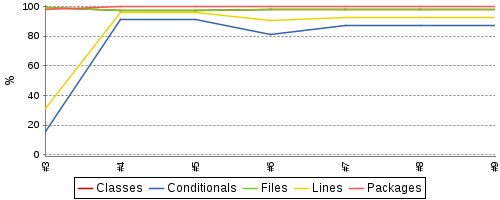
\includegraphics[scale=0.5]{/srv/sqa-reports/build/figs/graph_ooi-unittest.png}
\\
%\vspace{0.5em}
% Cobertura report (gantt chart)
%\textbf{Cobertura report}\par\medskip
\begin{ganttchart}[
    canvas/.append style={fill=none, draw=black!5, line width=.75pt},
    hgrid style/.style={draw=black!5, line width=.75pt},
    vgrid={*1{draw=black!5, line width=.75pt}},
    title/.style={draw=none, fill=none},
    %title label font=\bfseries\footnotesize,
    title label font=\normalsize,
    title label node/.append style={below=7pt},
    include title in canvas=false,
    bar label font=\mdseries\small\color{black!70},
    bar label node/.append style={left=2cm},
    bar/.append style={draw=none, fill=black!63},
    bar incomplete/.append style={fill=barblue},
    bar progress label font=\mdseries\footnotesize\color{black!70},
    group incomplete/.append style={fill=groupblue},
    group left shift=0,
    group right shift=0,
    group height=.5,
    group peaks tip position=0,
    group label node/.append style={left=.6cm},
    group progress label font=\bfseries\small,
    link/.style={-latex, line width=1.5pt, linkred},
    link label font=\scriptsize\bfseries,
    link label node/.append style={below left=-2pt and 0pt}
    ]{1}{5}
    \gantttitle{Cobertura Report}{-3} \\
    %\ganttgroup[progress=45]{Group 1}{1}{12} \\
            \ganttbar[progress=100.0]{Packages (8.0/8.0)}{1}{3} \\
            \ganttbar[progress=97.674416]{Files (42.0/43.0)}{1}{3} \\
            \ganttbar[progress=97.674416]{Classes (42.0/43.0)}{1}{3} \\
            \ganttbar[progress=92.79678]{Lines (2306.0/2485.0)}{1}{3} \\
            \ganttbar[progress=87.18411]{Conditionals (483.0/554.0)}{1}{3} \\
     [grid]
\end{ganttchart}
\end{center}

\subsection{Build status}
    Last build status on Jenkins CI \href{https://jenkins.indigo-datacloud.eu:8080//job/ooi-unittest/7}{ooi-unittest}.
    


\section{Functional/Integration testing}
\footnotesize
\textcolor{gray!90}{\textit{Functional testing must cover at least the basic functionalities that the product was requested to fulfill within the INDIGO-DataCloud project scope. Integration testing must cover the interactions with other components. Both types of testing will be automated whenever feasible by integrating them in the project's continuous integration service.}}
\normalsize
%\\[0.1in]

\label{sec:func_int_test}

    No functional or integration testing provided.
    
    


\section{GitBook documentation}
\footnotesize
\textcolor{gray!90}{\textit{Product-related documentation must be uploaded to GitBook's \texttt{indigo-dc} central repository. Types of documentation includes a) Developer b) Deployment and Administration c) Command-line Interface (CLI) and Application Program Interface (API) d) User Documentation. All these types may not be applied for every product. Those products that offer functionalities out of the scope of INDIGO-DataCloud project needs may not provide all the spectrum, but links to the
official documentation.}}
\normalsize
\\[0.1in]

\label{sec:gitbook}
Documentation available under \texttt{indigo-dc} GitBook organization: \vspace{0.1em} \begin{center}\url{https://indigo-dc.gitbooks.io/ooi/content/}\end{center} 
\subsection{Types of documentation currently provided}
\begin{center}
\graybox{\strut Readme}
\end{center}


\section{Configuration Management}
\footnotesize
\textcolor{gray!90}{\textit{Those products released by INDIGO-DataCloud project that need to be deployed by the end user must rely on a maintained open-source configuration management tool to provide an automated means to install and configure the product. The recommended tool is \texttt{Ansible}.}}
\normalsize
\\
%\\[0.1in]

\label{sec:configuration}

\begin{center}
\begin{tabular}{ll}
    Tool & \graybox{puppet} \\
    Deployment coverage & \graybox{installation/configuration} \\
    Manifest link & \url{https://github.com/indigo-dc/puppet-ooi} \\
\end{tabular}
\end{center}

\subsection{Build status}
\begin{center}
\begin{tabular}{ll}
        \href{None}{Ubuntu 14.04 LTS} & \redbox{failed}\\
        \href{None}{CentOS7} & \redbox{failed}\\
    \end{tabular}
\end{center}



\newpage

\part{How to read this document}
\setcounter{section}{0}

% Front/summary page
\section{Summary (front) page}
Both the overall product's SQA adherence and per-task status codes are explained below: \\
\begin{tabular}{l L{10cm}}
    \greenbox{COMPLETE} & Task has been successfully completed and fulfills the project's SQA requirements, listed in \href{https://owncloud.indigo-datacloud.eu/index.php/s/yDklCrWjKnjutVA}{Deliverable D3.1} and \href{https://    project.indigo-datacloud.eu/projects/wp3/wiki/Extensions_to_SQA}{Extensions to Software Quality Assurance} documents. \\ 
    \redbox{NOT COMPLETE} & Task has not been completed, yet some missing required bits have not been provided. \\
    \graybox{IN PROGRESS} & Task has not been completed, but can proceed as it is. \\[0.1em]
    \graybox{WP3 PENDING} & Task has some pending work from WP3 side, meaning that the product team already submitted the required data but it has not been yet consumed by WP3. \\
\end{tabular}



% Task progress
\section{Task Progress}


\subsection{Code style}
\begin{tabular}{l L{10cm}}
    \graybox{Code style definition} & Name and link of the standard to which the product is adhered. \\
    \graybox{Community/de-facto standard} & Whether the adopted standard is community-wide accepted. \\
    \graybox{Exceptions} & Number of exceptions from the standard definition. \\
    \graybox{Richness} & Number of rules defined in the adopted standard. Additionally (whenever available) the \graybox{number of errors}, \graybox{number of warnings} documented in the standard will be displayed as well as the \graybox{link} to the latest definition. \\
\end{tabular}


\subsection{Unit testing}
This section will display the a) \graybox{trend graph} with the evolution of the code coverage over time and b) the \graybox{Cobertura report}, with the coverage results of different methods. Both are taken from the project's Jenkins continuous integration service. \\
\textit{Note}: resultant coverage value is the lowest of the ones for the different methods: packages, files, classes, lines, conditionals.


\subsection{Functional/Integration testing}


\subsection{GitBook documentation}
Whenever the documentation of the product is available at the project's GitBook repository, both the a) \graybox{link} to the documentation index and b) \graybox{type of documentation} provided will be displayed in the report.


\subsection{Configuration Management}
Whenever the product has an recipe to be deployed automatically the following information will be available: \\[0.5em]
\begin{tabular}{l L{10cm}}
    \graybox{Tool} & Configuration management tool used. \\
    \graybox{Manifest link} & URL pointing to the manifest/s. \\
    \graybox{Deployment level} & Whether \texttt{installation}, \texttt{configuration} or both. \\
    \graybox{Build status} & Current build status for the project's supported OS distributions. \\
\end{tabular}


\end{document}